\documentclass[14pt]{article}
\usepackage
[
        a4paper,% other options: a3paper, a5paper, etc
        left=2cm,
        right=2cm,
        top=3cm,
        bottom=4cm,
]
{geometry}

\usepackage[utf8]{inputenc}
\usepackage{listings}
\usepackage{xcolor}
\usepackage{graphicx}
\lstset { %
    language=C++,
    backgroundcolor=\color{black!5}, % set backgroundcolor
    basicstyle=\footnotesize,% basic font setting
}


\title{Report.3.cuda}
\author{lehuyduc3 }
\date{November 2020}
\usepackage{indentfirst}
\parindent{}

\begin{document}

\maketitle

\section{How to implement labwork}
We use a loop to test the number of threads: from 1 to 256.
For each number of thread, we create enough block so that each pixel is processed by exactly 1 thread.
The kernel is as follow:

\begin{lstlisting}
__global__
void rgb2gray_labwork3(char* goutput, char* ginput, int pixelCount)
{
	const int i = blockIdx.x * blockDim.x + threadIdx.x;
	if (i < pixelCount) {
		goutput[i * 3] = (char)((int(ginput[i * 3]) 
		                        + int(ginput[i * 3 + 1]) 
		                        + int(ginput[i * 3 + 2])) / 3);
        goutput[i * 3 + 1] = goutput[i * 3];
        goutput[i * 3 + 2] = goutput[i * 3];        
	}
}
\end{lstlisting}

\section{Execution time and speedup}

\begin{figure}[h]
\centering
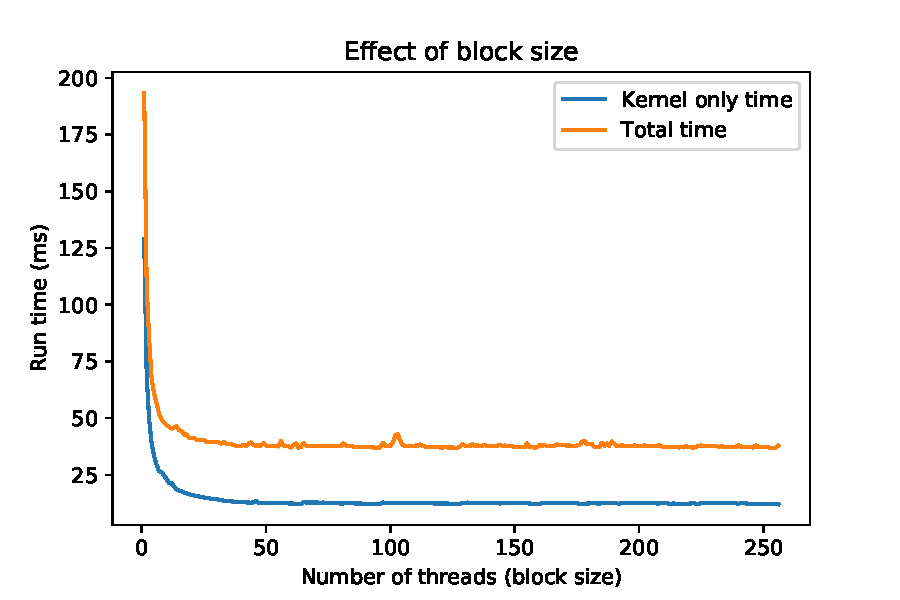
\includegraphics[scale=0.75]{report3_kerneltime.pdf}
\end{figure}

Kernel time stop improving after around 64 threads. At 64 threads, we have:
\begin{itemize}
    \item - Kernel time: 12.6ms
    \item - Total time: 37.2ms
    \item - CPU single-core: 96ms
\end{itemize}

So the total speed up is around 2.6x in total.

\end{document}
